\chapter{Marco Metodológico}
Para poder cumplir con los objetivos del proyecto fue necesario utilizar la metodología de desarrollo de software llamada \textit{Proceso Unificado de Rational} o RUP (por sus siglas en inglés) de IBM. A continuación se presentará brevemente la estructura de la metodología en cuestión, incluyendo sus fases y actividades asociadas.

\section{La metodología RUP}
El Proceso Unificado de Rational es un proceso de ingeniería el cual provee un enfoque disciplinado hacia la asignación de tareas dentro de una organización orientada al desarrollo. Su objetivo es asegurar la producción de software de alta calidad que cumpla con las necesidades de sus usuarios finales dentro de tiempo y presupuesto predecible. [Kru00]

El Proceso Unificado de Rational captura varias  de las \textit{mejores prácticas}  en el desarrollo de software moderno de una manera que se puedan adaptar  a una gama amplia de proyectos y organizaciones. Las (6) prácticas principales cubiertas por el proyecto son: 
\begin{enumerate}
\item Desarrollar software de manera iterativa.
\item Administrar requerimientos.
\item Utilizar arquitecturas basadas en componentes,.
\item Modelar el software de manera visual.
\item Verificar la calidad continuamente.
\item Mantener el control sobre los cambios realizados al software.
\end{enumerate}

La Figura x  muestra la arquitecutra general  del Proceso Unificado de Rational. El modelo esta compuesto por dos dimensiones: el horizontal representa el tiempo y se ven reflejados los distintos ciclos de vida del software a medida que este se va desarollando; mientras que en el eje vertical se reflejan los principales flujos de trabajo, los cuales se encargan de agrupar actividades segun su naturaleza.
Por otra parte, el eje horizontal representa el aspecto dinámico del software a medida que este es aplicado. Se ve reflejado en la forma de ciclos, fases, iteraciones e hitos. A su vez, el eje vertical muestra el aspecto estático del software, describiéndolo en términos de actividades, flujos de trabajo, artefactos y trabajadores. 

\section{Fases de RUP}
RUP divide el proceso de desarollo en cuatro fases. Dentro de cada fase se puede realizar una cantidad variable de iteraciones dependiendo de la envergadura del proyecto. Cada fase hace hincapié sobre distintas actividades asociadas al desarrollo del proyecto, y producen como resultado una serie de artefactos e hitos (que deben cumplirse) con la culminación de la fase. Las fases del proceso se discuten a continuación.
\begin{figure}[hbt]
\begin{center}
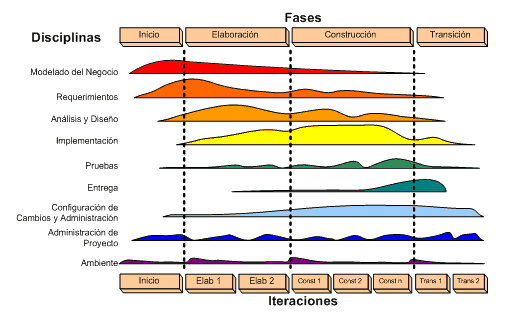
\includegraphics{RUP}
\caption{Arquitectura general del Proceso de Unificación Rational.}
\label{fig:figura1}  
\end{center}
\end{figure}

\subsection{Iniciación}
Es la primera fase del Proceso Unificado de Rational, en la cual el ímpetu inicial para Desarrollar software (una idea, un prototipo, una solicitud de propuesta, una evolución sobre una generación previa) se materializa hasta el punto de obtener el respaldo suficiente (al menos dentro de la organización) para poder entrar en la etapa de elaboración. [Kru00]
El objetivo principal de la fase de inciación es informar y mantener de acuerdo al público interesado (stakeholders) sobre los objetivos del ciclo de vida del proyecto. Otros objetivos de la fase incluyen:

\begin{itemize}
\item Establecer el alcance y condiciones límite del proyecto, incluyendo el concepto de operación, criterios de aceptación y descripciones sobre lo que se desea que contenga el producto.
\item Desarrollar los casos de uso críticos del sistema, es decir, aquellos escenarios principales que definirán la funcionalidad del proyecto y en los cuales se dedicará el mayor esfuerzo de desarrollo.
\item Estimar costos, tiempos de desarrollo y riesgos globales para el proyecto.
\end{itemize}

Los artefactos producidos para el cierre de la fase son los siguientes:

\begin{itemize}
\item Un documento de visión que muestre los principales requerimientos, funcionalidades y restricciones del proyecto.
\item Un modelo de casos de uso incial, en donde se muestren los casos de uso y actores que se pueden identificar para la fase en cuestión
\item Un glosario del proyecto inicial.
\item Una propuesta de negocio incial que incliya: el contexto del negocio, criterios de éxito y predicciones financieras.
\item Un plan de proyecto en donde se muestren las fases (e iteraciones) a llevarse a cabo.
\end{itemize}

El hito de la fase de inciación es la obtención y evaluación de los \textit{Objetivos del Ciclo de Vida} del proyecto. Al alcanzar este hito debe realizarse una serie de evaluaciones que deben cumplise satisfactoriamente antes de continuar a la próxima fase del proyecto. Con este hito se debe validar que las partes interesadas del proyecto hayan llegado a un acuerdo sobre el alcance del mismo y las estimaciones de costos y tiempo. Adicionalmente, se debe validar la compresión de requerimientos del cliente y que estos se vean plasmados en los casos de uso definidos. Por último, se debe validar la credibilidad de las prioridades y riesgos asociados al proceso de desarrollo.
De todos los hitos presentes en la metodología, este es considerado como el más importante, ya que su resultado puede llevar a la cancelación del proyecto o a que el mismo tenga que ser re-planteado.
\subsection{Elaboración}
Es la fase del proyecto orientada a terminar de definir la visión del producto y la arquitectura a utilizar. [Kru00] La fase de elaboración tiene como objetivo analizar los problemas asociados al dominio de la aplicación, establecer una arquitectura sólida para el producto, elaborar un plan de proyecto definitivo y eliminar la mayor cantidad de elementos de alto riesgo. Cada decisión con respecto a la arquitectura del producto deben hacerse teniendo un conocimiento pleno del alcance del producto, su funcionalidad principal  y requerimientos no funcionales (por ejemplo, requerimientos de desempeño).
Los objetivos principales de la fase son:
\begin{itemize}
\item Definir y validar la arquitectura del producto de la manera más  rápida posible.
\item Definir y validar la visión del proyecto.
\item Contruir un plan (de alta fidelidad) para la etapa de Construcción.
\item Demostrar que la arquitectura desarrollada pueda soportar la visión por un costo y un tiempo razonable.
\end{itemize}
Algunos artefactos como resultado de la ejecución de la fase se muestran a continuación:
\begin{itemize}
\item Un modelo de casos de uso completado un 80   
\end{itemize}
\subsection{Construcción}
\subsection{Transición}

\section{Fases contempladas para el proyecto}